\documentclass{article}

\usepackage[margin=1in]{geometry}
\usepackage{graphicx} 
\usepackage{gensymb}
\usepackage{amsmath}
\usepackage{multicol}
\usepackage[font=small,labelfont=bf]{caption}

\title{Filter}

\begin{document}
\begin{center}
    {\huge{Filter}}
\end{center}    
    \begin{multicols}{2}
    \section*{Problem}
    One problem we noticed in the samples generated by our model after the application of the filter is that some are really good and realistic, while others are 
    have no sense, for exemple let's take the samples shwon in the image below:
    \begin{center}
        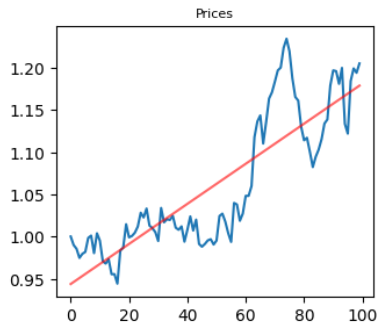
\includegraphics[scale=0.49]{imgs/serie_comp_1.png}
        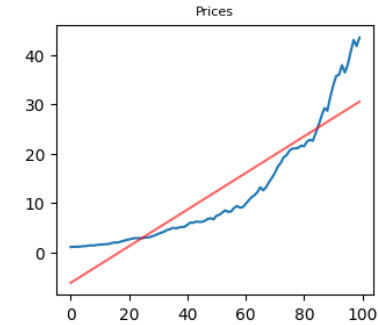
\includegraphics[scale=0.49]{imgs/serie_comp_2.png}
    \end{center}
    As we can see, the first series is very realistic while the other one is completly out of scale and shows a trend that is not 
    typical for fiancial time series. In order to solve this problem, we created a filter that selects from the samples generated the realistic series without modifyng the model output, so we end up with a realistic series dataset.
    \section*{How It works}
    To select the realistic series we came up with several metrics, the value of which can be tuned in the filter parameters:
    \paragraph*{Distance between residuals}
    We noticed that once we apply a linear regression to a series, the distance between consecutive residuals is smaller when the series shows an unrelistic behavior.
    In contrast, when we have a more realistic series the discance between consecutive points residuals is bigger.
    \begin{center}
        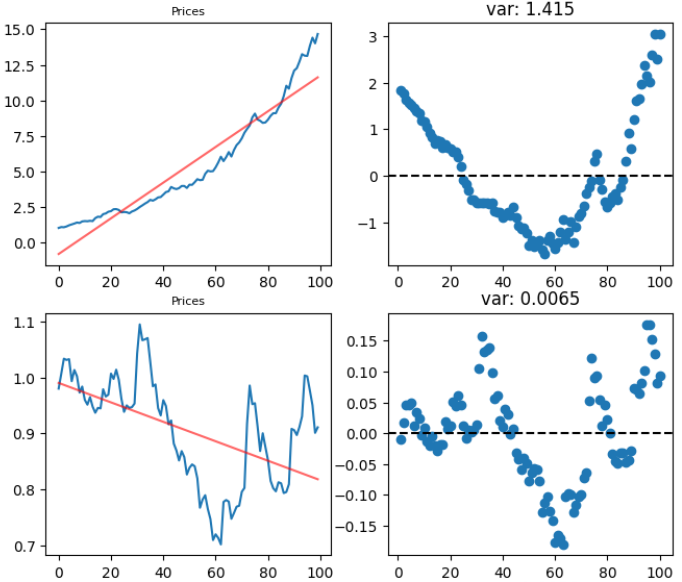
\includegraphics[scale=0.6]{imgs/2_res.png}
    \end{center}
    We scaled the price of the generated series between 0 and 1 to make it comparable and applied a linear regression to it. Once we obtained the linear regression, we computed the summation of the distance between consecutive residuals. 
    At this point, the filter just selects the series in which the summation of consecutive residuals is within a given threshold.\\
    \textbf{DfGenerator paramether}:  \textbf{variance\_th}.
    \paragraph*{Maximum range of oscillation}
    We decided to introcuce a parameter in the filter to chose the maximum range of oscillation between the first point an the last one in percentage. This is because we think it could be useful to have the freedom to decide the type of series we want 
    to generate to expand our dataset. Potentially we want to expand our dataset with very volatile series, in this case we can chose to use an hight max range of osscilation. Alternatively, our need could be to expand our dataset with more stable series, for example in order to decrease 
    the volatility of the predictions made by a model. In that case we can tune the parameter chosing a lower max range.\\
    \textbf{DfGenerator paramether}:  \textbf{max\_range}.

    \end{multicols}
    \newpage
    \begin{center}
        {\huge{Final Results}}
    \end{center} 
    The final result of the project is a program capable of generate realistic financial series such the following:
    \begin{center}
        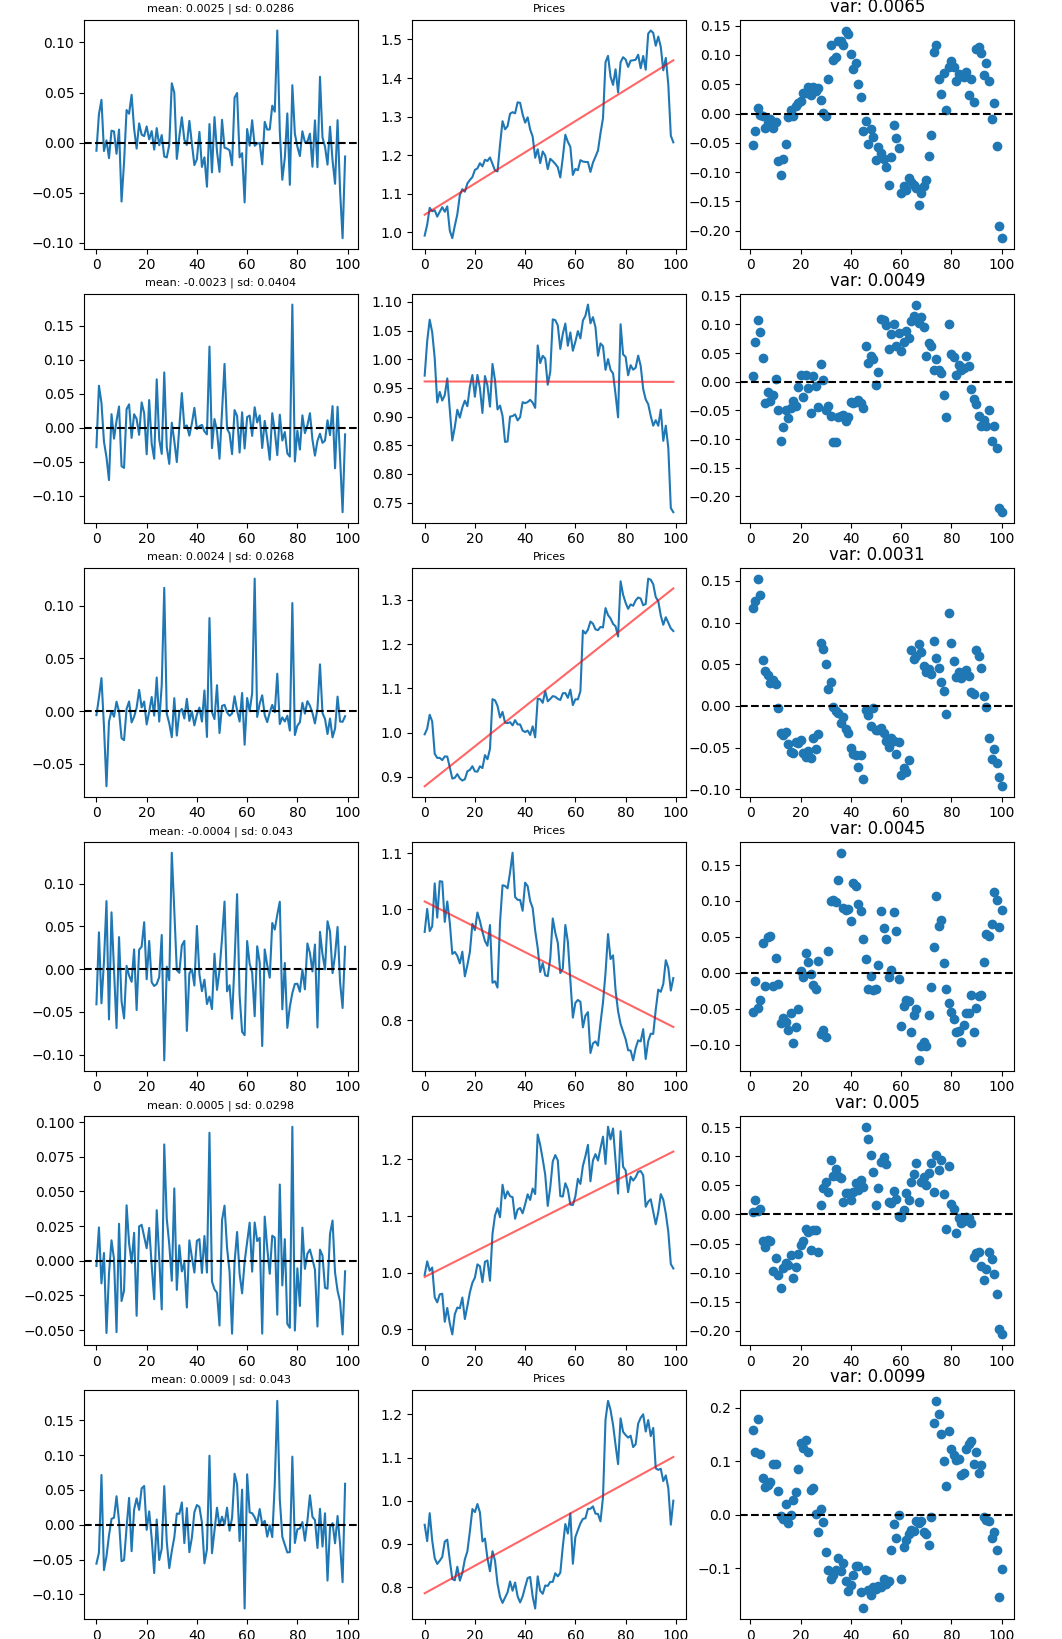
\includegraphics[scale=0.5]{imgs/results_reduced.png}
    \end{center}
    \newpage
    The generated series are visually similar to the original series. In the graph, the generated series are represented with a grey background to distinguish them from the original ones:
    \begin{center}
        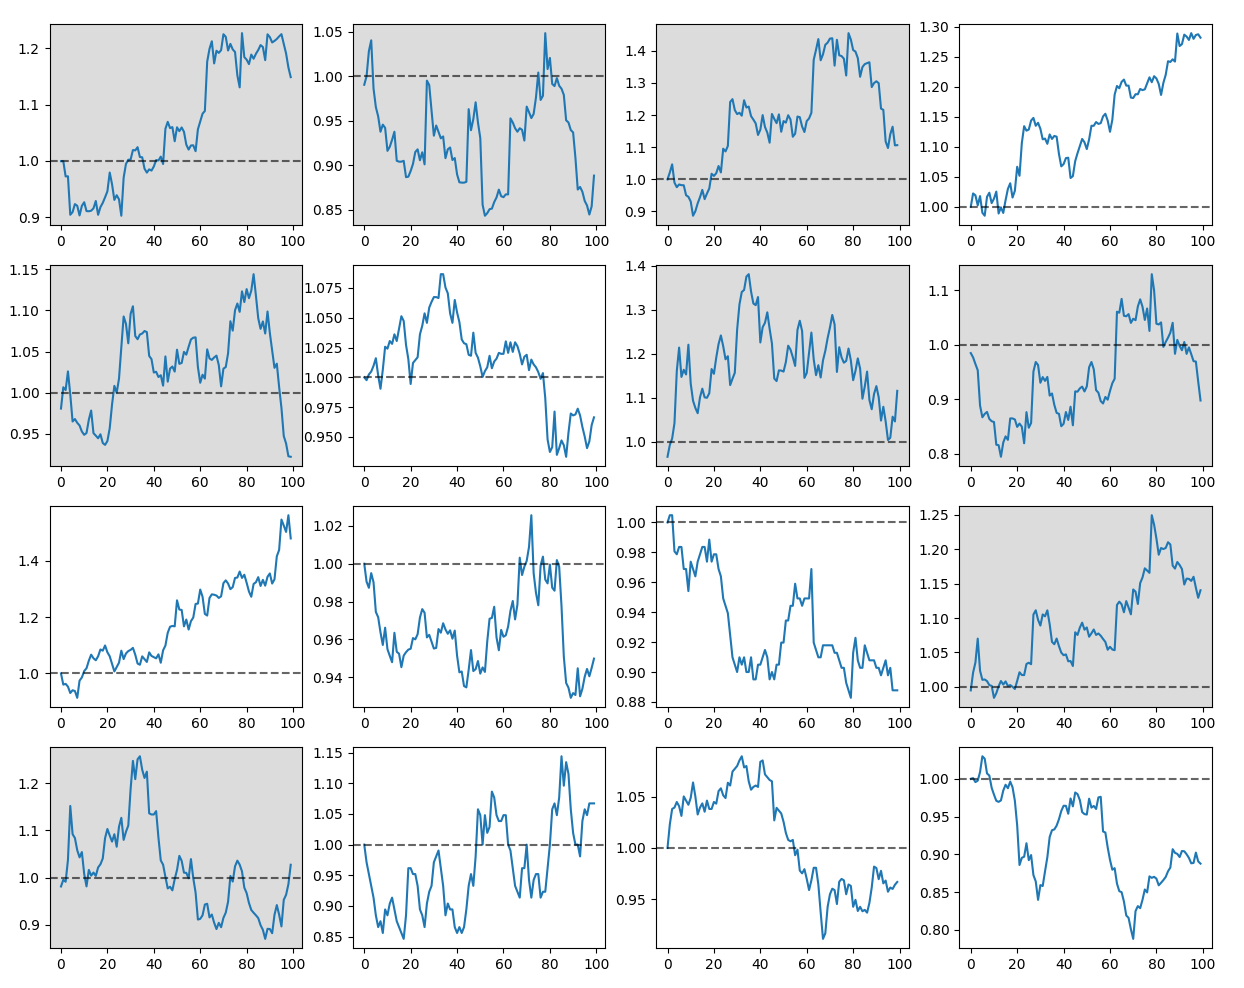
\includegraphics[scale=0.5]{imgs/series_comparison_README.png}
    \end{center}
    one of the main characteristic of retuns of financial series is the mean that is almost equal to 0. For that reason we tested if the mean of the returns generated by our model and the mean 
    of the real series of the dataset is the same. To do the following hypotesis test:
    \begin{equation}
        \begin{cases}
        H_0: \;\; \overline{X}=0\\
        H_1: \;\; \overline{X} \neq 0
    \end{cases}\,.
    \end{equation}
    $$T=\frac{\overline{X}-\mu_0}{S_n/\sqrt{n}} \;\;\;\;\;\;\;\;\;\;\; T|H_0 \sim t_{n-1}$$
    to test this hypothesis we generated a dataset of 10 000 samples an computed the mean: 0.00026567.
    \newpage
    The program takes approximatly 20 mintutes to generate a 10 000 samples dataset on a single cpu Intel Core I7. The distribution of the generated samples, looks like this:
    \begin{center}
        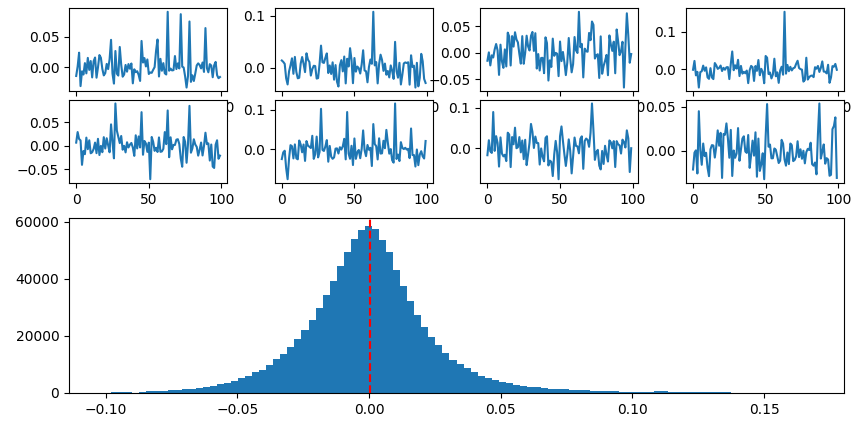
\includegraphics[scale=0.7]{imgs/generated.png}
    \end{center}

\end{document}
